\documentclass[a4paper,12pt,fleqn]{article}
\usepackage{fixltx2e}
\usepackage[utf8]{inputenc}
\usepackage{graphicx}
\usepackage{sidecap}
\usepackage{fancyhdr}
\usepackage{amssymb,mathtools}
\usepackage[swedish]{babel}
\usepackage[margin=1.5in]{geometry}
\usepackage{abstract}
\usepackage[parfill]{parskip}
\usepackage{tocloft}
\usepackage{adjustbox}
\usepackage{textcomp}
\usepackage[T1]{fontenc}
\usepackage{listings}
\usepackage{xcolor,colortbl}
\usepackage{hyperref}

%----------------------------------------------------------------
%C-kod formatering

\definecolor{listinggray}{gray}{0.9}
\definecolor{lbcolor}{rgb}{0.9,0.9,0.9}
\lstset{
backgroundcolor=\color{lbcolor},
    tabsize=4,    
%   rulecolor=,
    language=[GNU]C++,
        basicstyle=\scriptsize,
        upquote=true,
        aboveskip={1.5\baselineskip},
        columns=fixed,
        showstringspaces=false,
        extendedchars=false,
        breaklines=true,
        prebreak = \raisebox{0ex}[0ex][0ex]{\ensuremath{\hookleftarrow}},
        frame=single,
        numbers=left,
        showtabs=false,
        showspaces=false,
        showstringspaces=false,
        identifierstyle=\ttfamily,
        keywordstyle=\color[rgb]{0,0,1},
        commentstyle=\color[rgb]{0.026,0.112,0.095},
        stringstyle=\color[rgb]{0.627,0.126,0.941},
        numberstyle=\color[rgb]{0.205, 0.142, 0.73},
%        \lstdefinestyle{C++}{language=C++,style=numbers}’.
}
\lstset{
    backgroundcolor=\color{lbcolor},
    tabsize=4,
  language=C++,
  captionpos=b,
  tabsize=3,
  frame=lines,
  numbers=left,
  numberstyle=\tiny,
  numbersep=5pt,
  breaklines=true,
  showstringspaces=false,
  basicstyle=\footnotesize,
%  identifierstyle=\color{magenta},
  keywordstyle=\color[rgb]{0,0,1},
  commentstyle=\color{Darkgreen},
  stringstyle=\color{red}
  }
  %-----------------------------------------------------------------
  %marginaler

  \renewcommand{\abstractnamefont}{\normalfont\normalsize\bfseries}
  \renewcommand{\abstracttextfont}{\normalfont\small}
  \renewcommand{\headrulewidth}{0pt}
  \renewcommand{\cftsecleader}{\cftdotfill{\cftdotsep}} 
  \setlength{\absleftindent}{0pt}
  \setlength{\absrightindent}{0pt}
  \setlength{\headheight}{15pt}

  \addtolength{\oddsidemargin}{-.5in}
  	\addtolength{\evensidemargin}{-.5in}
  	\addtolength{\textwidth}{1in}


  %-----------------------------------------------------------------
  %header and footer

  \pagestyle{fancy}
  \lhead{
  	\begin{picture}(0,0)
  		\put(5,0){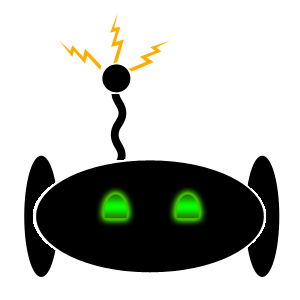
\includegraphics{logotyp.png}}
  	\end{picture}}
	
  \fancyhead[C]{\small{Mapmaster2001}}
  \fancyhead[R]{\small \today}
  \fancyfoot[L]{\small{TSEA56 \\ LIPS Kappa}}
  \fancyfoot[C]{\small{\thepage}}
  \fancyfoot[R]{\small{Projektgrupp 8 \\ mapmaster2001@cyd.liu.se}}

  %-----------------------------------------------------------------

%-------------------------------------------------------------------
%Första sidan

\begin{document}
	\pagestyle{fancy}
	 \pagenumbering{gobble}
	\vspace*{\fill}
		\begingroup
			\begin{center}
				\huge{\textbf{Simultan positionering och kartläggning}}
				\\
				\vspace{10pt}
				\normalsize
				Tobias Grundström och Hans-Filip Elo
				\\
				Kandidatprojekt Y - Grupp 8 - VT2014
				\\
				Version 0.1
				\end{center}
		\endgroup
	\vspace*{\fill}

	\begin{center} %Börjar centrering 
		Status
		\\
		\vspace{3pt} %Whitespace 3 pts
	    \begin{tabular}{| p{3cm} | p{3cm} | p{3cm} |} %tabell, 4 horizontella |, 3 cm emellan dem.
	    \hline %översta horizontella linjen.
	    Granskad & - & \today \\ \hline % & -tecken för att "gå till nästa ruta" 
		Godkänd & - & - \\ \hline % avslutas med \\ och \hline.

	    \end{tabular}
	\end{center}
	\vspace{2cm}
	\newpage
%-----------------------------------------------------------------
%Projektidentitet


	\vspace*{\fill}
		\begingroup
			\begin{center}
				\pagenumbering{roman}
				\LARGE{\textbf{PROJEKTIDENTITET}}
				\\
				\footnotesize
				Grupp 8, 2014/VT, MapMaster2001
				\\
				Linköpings tekniska högskola, Institutionen för Systemteknik (ISY)
				\\
				\vspace{1cm}
	  \begin{tabular}{| p{3cm} | p{4.3cm} | p{2.4cm} | p{3.8cm} |}
	    \hline
		\textbf{Namn} & \textbf{Ansvar} & \textbf{Telefon} & \textbf{E-post} \\ \hline
	    Jens Edhammer & Dokumentanvsvarig (DOK) & 076-030 67 80 & jened502@student.liu.se \\ \hline
		Erik Ekelund & Designansvarig (DES) & 073-682 43 06 & eriek984@student.liu.se \\ \hline
		David Habrman &  & 976-017 71 15 & davha227@student.liu.se \\ \hline 
		Tobias Grundström & Testansvarig (TES) & 073-830 44 45 & tobgr602@student.liu.se \\ \hline 
		Hans-Filip Elo &   & 073-385 22 32 & hanel742@student.liu.se \\ \hline 
		Niklas Ericson & Projektledare (PL) & 073-052 27 05 & niker917@student.liu.se \\ \hline
	    \end{tabular}

		\vspace{1cm}
		\textbf{E-postlista för hela gruppen:} mapmaster2001@cyd.liu.se
		\\[0.5cm]

		\textbf{Kund}: Mattias Krysander, Linköpings universitet, 581 83  LINKÖPING, \\
		013-28 21 98, matkr@isy.liu.se \\
		\textbf{Kontaktperson hos kund}: Mattias Krysander, 013-28 21 98,matkr@isy.liu.se 
		\\
		\textbf{Kursansvarig}: Tomas Svensson, 3B:528,013 28 21 59,tomass@isy.liu.se
		\\[0.5cm]
		\textbf{Handledare}: Peter Johansson, 013-28 1345 peter.a.johansson@liu.se

				\end{center}
		\endgroup
	\vspace*{\fill}
\newpage

%-----------------------------------------------------------------
%Innehållsföreteckning

\addto\captionsswedish{\renewcommand{\contentsname}{Innehållsförteckning}}

\tableofcontents
\thispagestyle{fancy}
\newpage

\pagenumbering{arabic}
%-----------------------------------------------------------------
%Översikt

%------------------------------------------------
%--------------------Inledning-------------------
%------------------------------------------------
\section{Inledning}

Simultan positionering och kartläggning (SLAM) är ett problem som kan liknas vid ''Hönan och ägget''-problemet. Utan att veta var vi är - hur kartlägger vi då vår omgivining? Åt andra hållet får man ställa sig frågan - hur kartlägger vi vår omgivning utan att veta var vi är? 

Det är inte helt enkelt att lösa dessa frågor, men det finns approximativa lösningar på problemet SLAM. Gemensamt för alla lösningar är att de bygger på möjligheten att läsa av sin omgivning i kombination med
sannolikhetsteori. Då sensordata aldrig kan antas vara exakt använder man sannolikhetsteori för att göra rimlighetsbedömningar i de stickprov av sensordata som sensorerna ger oss.

Själva problemet är alltså inte entydigt löst rent matematiskt, utan
bygger på sannolikhetsteori i kombination med att moderna processorer
och minnen kan hantera en stor mängd data. Moderna processorer möjliggör
alltså ett stort stickprov vilket kan leda till en mindre osäkerhet.

\subsection{Syfte}
Syftet med denna rapport är att fördjupa läsaren i de algoritmer och tekniker som används för kartläggning och positionsbestämning hos ett icke-medvetande system och att lösa ett enklare SLAM-problem.

\subsection{Historia}

Principerna för SLAM formulerades för första gången 1986\footnote{Smith, R.C.; Cheeseman, P. (1986).
''On the Representation and Estimation of Spatial Uncertainty''. The
International Journal of Robotics Research, 5(4), sida 56–68. Hämtad 28 mars 2014}. Redan vid formuleringen av problemet beskrevs SLAM som en inexakt vetenskap. SLAM handlar om att skaffa sig en approximativ uppfattning av sin omgivning och position som är tillräckligt bra för att fatta ett beslut kring färdväg och/eller kartläggning. 

Utvecklingen på området har sedan dess accelererat kraftigt tack vare
mikrokontrollers förmåga att hantera mer data - eftersom
sannolikhetsberäkningarna SLAM innefattar gynnas kraftigt av att arbeta
med stora stickprov.

På senare år har man, precis som inom många andra vetenskapliga områden, sett utvecklingen ta ytterligare ett kliv tack vare internet och öppna källkodsprojekt som Github och OpenSLAM. Att göra en sökning på ''SLAM'' på Github resulterar i en mängd aktiva projekt på området. Eftersom källkoden där också finns tillgänglig är detta ett utmärkt exempel för de som vill läsa på om SLAM-algoritmer. 

%------------------------------------------------
%-------------Problemformulering-----------------
%------------------------------------------------

\section{Problemformulering}

En robot med tillgång till ett antal avståndssensorer, ett gyro och en RFID-sensor placeras i ett stängt område med dimension 6x6 meter och som är uppdelad i 40x40 centimeters segment. Den ska, med en vägg som startpunkt, helt autonomt kartlägga området genom att markera ut var väggar finns och var det finns områden som inte går att nå. Den ska även markera ut var det går att finna RFID-taggar. Om inte hela det slutna området är kartlagt ska den upptäcka vilka segment som är oupptäckta, färdas dit och lägga till det i kartan. När området är kartlagt ska roboten ta sig tillbaka till startpunkten och avsluta arbetet. 

\subsection{Tillgängligt materiel}

I världen finns ett väldigt stort utbud av hårdvara, mjukvara och kommunikationslänkar. Denna rapport begränsar sig till kod som kan köras på AVR-processorer, och då mer specifikt Atmega 1284p\footnote{ISY, https://docs.isy.liu.se/twiki/pub/VanHeden/DataSheets/atmega1284p.pdf}

ISY tillhandahåller följande i sin utvecklingsmiljö: 
\begin{itemize}
	\item Atmega 1284p-processorer
	\item Utvecklingsmiljön Atmel Studio med kompilatorn avr-gcc
\end{itemize}

%------------------------------------------------
%--------------------Kunskapsbas-----------------
%------------------------------------------------
\section{Kunskapsbas}

%----------------------Odometri------------------
\subsection{Odometri}

För att kunna utföra SLAM krävs det att man gör odometri, d v s kontinuerligt uppskattar vägen man färdats. Odometri kan göras på olika sätt - exempelvis genom att optiskt mäta avstånd till objekt i sin omgivning, vinkelhastigheter på hjul med känd storlek eller steg med given längd. 

Uppskattandet av färdvägen är aldrig en exakt lära. Det finns alltid en viss osäkerhet i sensorer. Det är av denna anledning som SLAM är en sannolikhetslära mer än en exakt vetenskap. 

Många robotar nyttjar förmågan att optiskt mäta objekt i sin omgivning, men det förekommer även implementeringar med radar och sonar. Det finns då möjlighet att kompensera för tidigare mätfel vid framtida mätningar, något som inte bara går att utföra med data från optiska sensorer, men som kan göra större inverkan på dessa. Om man enbart förlitar sig på interna mätningar finns risken att tidiga mätfel görs, vilket fortplantar sig och leder till än större felskattningar senare under kartläggningen. 

Med optisk avläsning av omvärlden finns alltid möjligheten att korrigera tidigare felaktiga mätvärden genom att samla in mer mätdata för att mer korrekt kunna beskriva sin omgivning. Av den anledningen är all typ av SLAM beroende av att på något sätt granska sin omgivning. 

\subsubsection{Tillståndsrepresentation av reglersystem}

Inom reglerteknik kan linjära system beskrivas på så kallad tillståndsformel så som Glad, Torkel och Ljung, Lennart (2006) beskriver i \textit{Reglerteknik - Grundläggande teori}. I fallet med SLAM använder man lämpligen sensorernas värden som tillstånd, tecknat $\vec{x}$. Tillstånden mäts med diskreta värden då datorer endast hanterar diskreta mätningar och ej kontinuerliga. En diskret tillståndsbeskrivning av ett linjärt reglersystem beskrivs av: 

\begin{gather}
\vec{x}[n+1] = A\vec{x}[n] + B\vec{u}[n] \\
\vec{y}[n] = C\vec{x[n]} + D\vec{u[n]}
\end{gather}
\\
Där A, B, C och D är insignaler, u är insignaler och $\vec{y}$ exempelvis är kringliggande objekts position i förhållande till till roboten, alternativt robotens position. 

I ett realiserbart system nyttjas sensorer med en viss osäkerhet. Man kan därmed enbart skatta systemets tillstånd och inte exakt beräkna dem. 

Tillståndsvariablerna kan skattas med flera metoder utifrån tillgänglig mätdata. Två exempel på väl använda metoder Maximum likelihood-metoden (ML-skattning) och Minstakvadratmetoden. Minstakvadratmetoden är något precisare - medan implementeringen av ML-skattning är enklare. Då man bygger en robot som implementerar SLAM är det ofta lämpligt att implementera ML-skattning. 

\paragraph{ML-skattning}

Antag att en sensors mäter en längd. Längdens korrekta värde ges av $x_true$, och att $\hat{x} $ är ett givet stickprov, alltså mätdata, med N antal mätningar. 

Det mest sannolika värdet fås, för diskreta mätvärden, binomialfördelningen. 

\begin{gather}
P(X = x_{i}) = p^{x_{i}}(1-p)^{n-x_{i}}
\end{gather}

Där p är sannolikheten att sensorvärdet är $x_i$ och n är antalet mätningar med resultat $x_i$. 

Sannolikhetsfunktionen, L, för hela stickprovet ges sedan av: 

\begin{gather}
L = \prod\limits_1^i{p^{x_{i}}(1-p)^{n-x_{i}}}
\end{gather}

Det mest sannolika värdet fås då $\frac{dL}{dp}$ är lika med 0. För att förenkla derivering och beräkningar används $log(L)$. Multiplikationssumman blir då en vanlig summa. 

\begin{gather}
\log(L) = \sum\limits_1^i{\log{(p)}{\cdot}x_{i}+\log{(1-p)}\cdot{(n-x_{i})}}
\end{gather}

Derivatan ges sedan av: 

\begin{gather}
\frac{dL}{dp} = 0 = \sum\limits_1^i{\frac{x_i}{p}+\frac{n-x_i}{1-p}}
\end{gather}

Vilket efter uträkningar ger $p = \bar{x}$. Vid ML-skattning av sensorvärden är alltså medelvärdet av sensordata lämpligt att använda.

\subsubsection{Filtrering av sensordata}

Inom odometri finns det några olika tekniker för att filtrera sensordata från sin omgivning och besluta om var inom given inertialram sin nuvarande position är. Gemensamt för samtliga tekniker är att de är filter som arbetar mot oberoende tillståndsvariabler. 





%-------------------------------Typer av SLAM--------------------------------------------------------------------------------
\subsection{Typer av SLAM}
Det finns olika typer av SLAM för olika typer av tillämpningar och med olika egenskaper. Vissa är bra på större avstånd medan andra är mer precisa och bra på kortare avstånd. 

\subsubsection{Kalmanfilter (KF-SLAM)}
Ett Kalmanfilter är en typ av algoritm som med hjälp av tidigare mätdata från sensorer som kan innehålla brus och störningar uppskattar okända variabler. Ett Kalmanfilter arbetar på linjära och oberoende tillståndsvariabler och är ett essentiellt verktyg för vägval samt positionsuppskattningen i ett SLAM-system. 

Kalmnafilter är en lösning

\subsubsection{EKF-SLAM} 
EKF-SLAM är en förkortning för Extended Kalman Filter for Simultaneous Localization And Mapping. Det utökade Kalmanfiltret (extended) skiljer sig från det ursprungliga på så vis att den används vid icke-linjära förhållanden och istället linjäriserar variablerna kring ett medelvärde och deras kovarians. Med kovarians menas då hur de olika variablerna beror av varandra.

Algoritmen arbetar oftast i två steg; först skattas variablerna sedan vid nästa mätning 
kommer de skattade variablerna viktas, där de med mest säkerhet är av störst vikt.

\subsubsection{FastSLAM}
FastSlam är en teknik där systemet visuellt kan uppfatta landmärken. Landmärkenas position i förhållande till roboten noteras och uppmäts med regelbundna samplingar. Genom att positionsbestämma dessa landmärken kan roboten snabbare bestämma sin position. 

FastSLAM är snabbare på att bestämma sin position än KF-SLAM men är däremot inte genomförbar då miljön systemet rör sig i är så pass homogen att inga landmärken går att utfinna. Om vi tar den bana vår robot ska kartlägga som referens är den väldigt homogen\footnote{Tävlingsregler: \url{https://drive.google.com/file/d/0B758zzcy4ZrTeG1wRTY4WG9lTDQ/edit?usp=sharing, Hämtad 28 mars 2014}}. fastSLAM är antagligen inte den bästa tekniken för positionsbestämning och kartläggning av den typen av ''rum''. 



\subsubsection{VSLAM}

VSLAM står för visuell SLAM, vilket betyder att lokaliseringen sker med hjälp av kameror. Kamerorna används för att finna landmärken i området som kartläggs och sedan använda dessa som referenser när roboten fortsätter att utforska för att t ex se hur långt och i vilken riktning förflyttning sker relativt landmärket. Visuell SLAM är en förutsättning för att utnyttja den tidigare nämna fastSLAM-tekniken. 

För att bedöma avstånd till ett objekt mäts vinklar mellan farkost och objektet vid olika tidpunkter. Utifrån farkostens hastighet kan mjukvaran sedan bestämma avståndet till objektet i fråga. 

VSLAM är i de allra flesta fall komplicerat att implementera då man behöver avancerade bildsökningsalgoritmer för att finna lämpliga landmärken. 

\subsubsection{TSLAM}
Tactile SLAM är en metod som provats för robotar vid kartläggning av ett mörklagt område. Metoden använder sig av känselsensorer för att hitta avgränsningar i området och med hjälp av detta rita upp kartan. Denna metod ger dock inte så bra resultat med de tekniker som existerar i dag.

\subsubsection{WiFi-SLAM}
Denna metod använder sig av styrkan på WiFi-signaler i närheten för att avgöra positionen. Detta är något som använts på t.ex. mobiltelefoner för att avgöra var personer befinner sig. 

För att WiFi-SLAM ska fungera krävs att accesspunkten har information om positionsdata för sig själv, alternativt att den anslutna enheten har information om var aktuellt WiFi är tillgängligt. I en mobiltelefon används den senare metoden då telefonen kan kontrollera var WiFi-nätverket finns med hjälp av GPS. 

\subsection{Implementeringar}

Det finns många exempel på implementeringar av SLAM. Robotdammsugare är ett bra exempel på en modern tillämpning som kan använda sig av SLAM. Det är då en liten enhet som kan använda sig av en modifierad version av VSLAM som kallas CV-SLAM. Detta står för Ceiling Visual SLAM, det vill säga att roboten har kameror som är riktade uppåt och använder landmärken i taket för att rita upp en karta över rummet den städar, så att den dammsuger alla platser i rummet istället för att städa samma punkt flera gånger. 

Det här är ett bra exempel på hur moderna, små mikrokontrollers kan möjliggöra SLAM att användas för att förenkla vår vardag.  

SLAM används, och har används under längre tid, till exempel också i rymdexpeditioner där robotar skickas upp i rymden för att upptäcka och kartlägga ställen som vi människor inte har möjlighet att besöka. 

%------------------------------------------------
%--------------------Fördjupning-----------------
%------------------------------------------------
\newpage
\section{Fördjupning och kodexempel}

För att rita en karta krävs det att mjukvara och hårdvara sammarbetar. Sensorerna och deras värden behöver översättas till något som kan behandlas av en dator. 

% --------------------------------------

\subsection{Skattning av parametrar}

I just detta problem, som är begränsat kommer positionen att skattas med hjälp av sensorvärden i form av vinkel och avstånd i kombination med enkla algoritmer. Eftersom en del parametrar är kända blir skattningen något lättare än om det hade varit t ex ett godtyckligt stort område. Det kommer att finnas två stycken tre-meters avståndssensorer som är riktade framåt och bakåt, här kallade $S_{front}$ \& $S_{back}$. Om båda sensorerna ger utslag på över tre meter kommer antagandet göras att de har gått utanför sitt mätområde och kommer då skattas som nedan. Mätvärdena kommer i största möjliga mån plockas ut som medelvärdet av den senaste mätdatan.

\begin{gather}
	S_{front}=3,00 m \\
	S_{back}=3,00 m
\end{gather}

Om endast den ena av sensorerna, i detta exempel $S_{back}$, befinner sig utanför sitt mätområde kommer den att skattas med hjälp av nedanstående ekvation. Om istället $S_{front}$ är okänd kommer den skattas på samma sätt. 

\begin{gather}
	S_{back}=6,00-S_{front}
\end{gather}

Där 6,00 m är den maximala längden som kan uppstå i området. Dessa sensorvärden kommer sedan användas för att skatta robotens position.


% --------------------------------------

\subsection{Positionsskattning}

För att uppskatta hur långt roboten har färdats kommer referensvärden på sensorerna sparas undan innan roboten rör sig. Dessa värden kommer sedan uppdateras varje gång roboten har färdats 40 cm (ett segment av området). För att veta när roboten färdats 40 cm kommer ett nuvarande sensorvärde jämföras med referensen t ex om roboten färdas framåt kommer differensen mellan $S_{front}$ \& $S_{frontref}$ beräknas. Förflyttningen har åstadkommits då ekvationen nedan är uppfylld. 

\begin{gather}
	S_{frontref} - S_{front} = 40
\end{gather}

% --------------------------------------

\subsection{Kartabstraktion}

En karta kan abstraheras i form av en rektangel med ett rutnät med dimensionen 33x17 rutor med koordinaterna (0,0) i det övre vänstra hörnet. Det definierade området i problemformuleringen, d v s det verkliga området skulle med liknande rutnät bli 15x15 rutor, men den utökas något för att underlätta uppritningen. Felaktigheter i avläsning kan leda till att roboten i abstraktionen tillfälligt är utanför sitt givna område. Roboten kommer i början att placeras i punkten (16,0) och rita upp kartan utifrån detta. Det kommer då inte spela någon roll hur roboten är placerad i det verkliga systemet eftersom det finns utrymma för 15 rutor åt båda hållen inklusive marginaler. 

Hur skapar man då en matris i mjukvara? Beroende på språk, utvecklingsmiljö och abstraktionslager/bilbiotek görs det såklart med olika syntax - men den övergripande designen är densamma oberoende av utvecklingsmiljö. 

En abstraktion av en matris i mjukvara skapas med hjälp utav nästlade arrayer, eller någon modern motsvarighet. I utvecklingsmiljön Atmel Studio finns språket C++ tillgängligt, men däremot ej C++ standardbibliotek med abstraktioner. I den här rapporten kommer vi därför att behandla arrayer istället för vektorer som kanske är vanligare i C++. 

\paragraph{Objektklasser}
~\\
Kartmatrisen hålls inne i en containerklass med funktioner för att abstrahera acess till den. I modern programmering är objekthantering ett kraftfullt verktyg för abstraktion. Klasser tänkbara att implementera för SLAM följer nedan, med engelska namnet inom parantes. Detta då programmering görs bäst på engelska tack vare att språken härstammar från engelskan. 

\begin{itemize}
	\item Karta (Map)
	\item Kartsektion (MapSection)
	\item Robot (Robot)
\end{itemize}

I en C++-implementering är Robot en dotterklass till MapSection. Detta då alla objekt i en matris måste vara av samma objekttyp. Roboten ärver då vissa egenskaper från MapSection - men innehåller klart mer logik för att hantera positionering och kartläggning. 

MapSection kan anta ett antal olika tillstånd för att markera vilken typ av område det är. Nedan följer några tänkbara tillstånd att implementera i klassen MapSection: 

\begin{itemize}
	\item Stängt område (Closed)
	\item Outforskat område (Unexplored)
	\item Tomt område (Empty)
\end{itemize}

Till en början är alla områden outforskade. I takt med att sensordata kommer in och beräknas kan sedan roboten omvandla tillstånden hos objekten i kartan utefter given logik. 

% --------------------------------------

\subsection{Kartläggningsalgoritmer}

Antag att roboten har en kartabstraktion, kan ta in sensordata och göra en uppskattning av sin omgivning - hur implementerar man sedan en bra och snabb kartläggningsalgoritm? Hur ska man utforska sin omgivning och i vilken ordning? 

Beroende på hur omgivningen ser ut finns det olika svar på frågan. Omfattningen för den här rapporten gäller insidan av ett rum i en byggnad, där alla hörn kan antas vara ortogonala. En enkel implementering är då att enbart köra roboten i ett rutnät - med ortogonala sökriktningar. Detta förenklar markant implementeringen då vinklar enbart behöver mätas vid rotationer, alltså riktningsändringar, istället för konstant under körning. En enkel implementering är ofta också en snabb implementering, både att realisera och att optimera. 

Nedan syns ett flödesschema över hur en tänkt kartläggningsalgoritm skulle kunna se ut. Kartläggningalgoritmen utför sina kommandon genom att anropa funktioner i Robotobjektet. Robotobjektet kan ses som operationens hjärna medan algoritmen är den övergripande handen som ser till att roboten arbetar i rätt ordning. 

\begin{figure}[htp] %Placera här om det finns plats, annars så snart som möjligt, på toppen av en sida.
  \begin{center}
  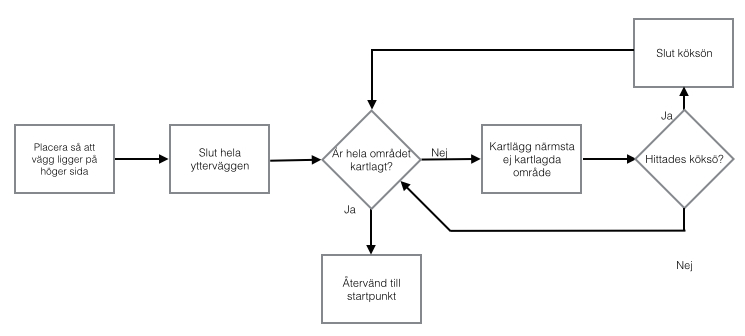
\includegraphics[keepaspectratio=true,scale=0.5]{../../Designspec/Flode_kartritning.jpg}  %skala och filnamn. 
  \end{center}
  \caption{Flödesschema kartläggning} %figurtext.
  \label{fig:fire} %glöm inte att uppdatera era labels
\end{figure}

%------------------------------------------------
%------------Resultat och slutsatser-------------
%------------------------------------------------
\newpage
\section{Resultat och slutsatser}

Till slut kan vi konstatera att SLAM används i många tillämpningar man kanske inte tänker på. Man kan också konstatera att algoritmerna, filtren och mjukvaran som används för att implementera SLAM är relativt komplicerade. Vi inser att vi gjort ett klokt beslut att fördjupa oss i just SLAM, då vi är beroende av detta i vårt projekt att konstruera en kartritande robot. 

% --------------- Källförteckning ---------------------
\newpage \section{Källförteckning} Smith, R.C.; Cheeseman, P. (1986).
''On the Representation and Estimation of Spatial Uncertainty''. The
International Journal of Robotics Research, 5(4), sida 56–68. Hämtad
28 mars 2014:
\url{http://www.frc.ri.cmu.edu/~hpm/project.archive/reference.file/Smith&Cheeseman.pdf}

Glad, Torkel och Ljung, Lennart. 2006. \textit{Reglerteknik - Grundläggande teori}. Upplaga 4:10. Lund. Studentlitteratur AB.

Risgaard, S; Blas, M.R (2005).
''SLAM for Dummies, A Tutorial Approach to Simultaneous Localization and Mapping''. 
Hämtad 28 mars 2014:
\url{http://ocw.mit.edu/courses/aeronautics-and-astronautics/16-412j-cognitive-robotics-spring-2005/projects/1aslam_blas_repo.pdf}

Karlsson, N.; Goncalves, L.; Munich, M.E.; Pirjanian, P.
''The vSLAM Algorithm for Navigation in Natural Environments''. Evolution Robotics, Inc. Hämtad 28 mars 2014:
\url{http://www.vision.caltech.edu/mariomu/research/papers/vSLAM-krs.pdf}

Fox, C.; Evans, M.; Pearson, M.; Prescott, T. (2012)
''Tactile SLAM with a biomimetic whiskered robot''. 2012 IEEE International Conference on Robotics and Automation. Hämtad 28 mars 2014.
\url{http://ieeexplore.ieee.org/stamp/stamp.jsp?tp=&arnumber=6224813}

FastSLAM: A Factored Solution to the Simultaneous
Localization and Mapping Problem, Stanford University. Hämtad 28 mars 2014.
\url{http://robots.stanford.edu/papers/montemerlo.fastslam-tr.pdf}

Openslam.org
\url{http://www.openslam.org/}

Atmega 1284p, Vanheden, databladsserver hos Institutionen för Systemteknik vid Linköpings Universitet. Hämtad 14 april 2014. \url{https://docs.isy.liu.se/twiki/pub/VanHeden/DataSheets/atmega1284p.pdf}

Kandidatprojekt Y: Elektronikprojekt, Tävlingsregler för katläggningsrobot. Hämtad 28 mars 2014.  \url{https://drive.google.com/file/d/0B758zzcy4ZrTeG1wRTY4WG9lTDQ/edit?usp=sharing}

% ----------------------------- Appendix
% -----------------------------------------
% 
\newpage \appendix \pagestyle{empty}
\newgeometry{left=2cm,right=2cm,bottom=2cm,top=2cm} \section{Appendix A}

\end{document}